\section{Tarpojien minihaikki}


\noindent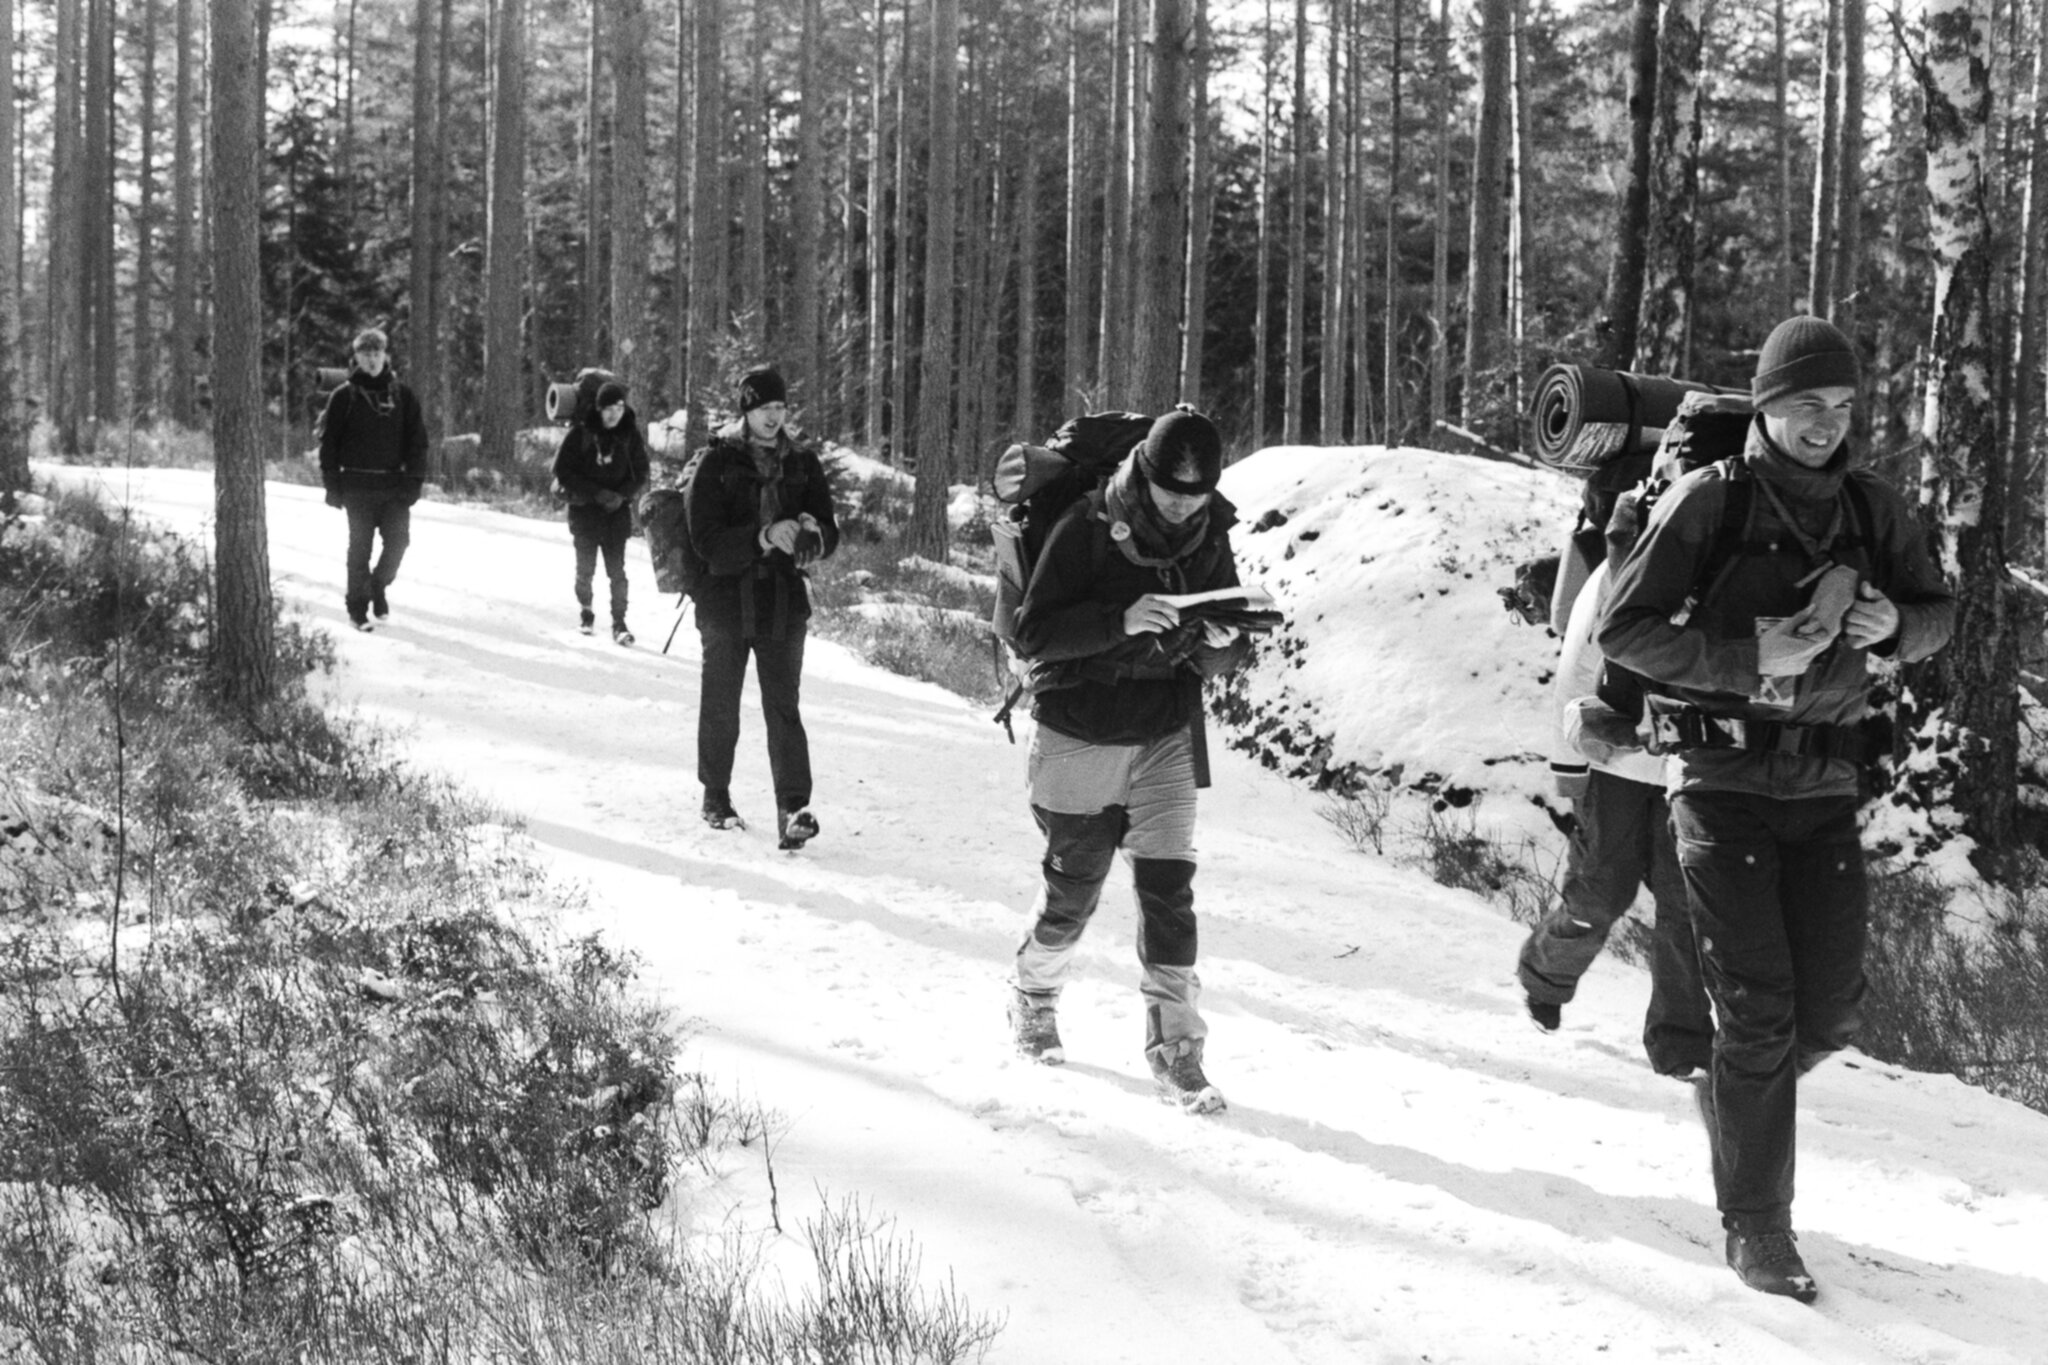
\includegraphics[width=1.0\linewidth,trim={0 0 0 1cm},clip]{assets/minihaikki4}

\begin{multicols}{2}

\noindent Perjantaina 14. maaliskuuta seitsemän rusakkoa lähti kohti Nuuksion
kansallispuistoa viettämään mukavaa viikonloppua pienimuotoisen vaelluksen
merkeissä. Vaikka vaellus oli nimensä mukaisesti tarpojille suunnattu, lopulta
matkaan lähti vain kolme tarpojaa, Alden, Jetro ja Tesla, sekä neljä johtajaa,
Ahti, Janne, Leo ja Tanguy. Retkikunta Leoa ja Jetroa lukuunottamatta lähti
liikkeelle kello 17.00 Kontulasta, Mikaelinkirkolta. Kontulasta hypättiin
metroon suuntana Rautatientori, josta matka jatkui E-junalla kohti Espoon
keskusta. Leo ja Jetro hyppäsivät junan kyytiin Huopalahden asemalta ja näin
koko retkikunta olikin kasassa! Junassa suoritettiin yhteisten varusteiden
jakoa, nautittiin matkaevästä ja manailtiin seuraavan yön sääennustetta, joka
lupaili jopa 9 asteen pakkasta. Onneksi kaikilla oli varusteet kunnossa,
jolloin kylmyys ei pääsisi haittaamaan! Junamatkan päätteeksi saavuttiin Espoon
keskukseen, josta bussi 245A lähti kuljettamaan retkeilijöitä kohti
kansallispuistoa. Bussimatka kesti kaikkiaan noin 20 minuuttia, minkä jälkeen
retkikunta jäi pois Kaitakorven bussipysäkillä. 

Ensimmäisen noin kahden kilometrin etapin suunnistamisen sai vastuulleen Jetro,
jonka tehtävänä oli suunnistaa porukka Hynkänlammen leiripaikalle. Reitti
Kaitakorvelta Hynkänlammelle kulki läpi Nuuksion ratsastuskeskuksen tilusten.
Hevosaitauksen vieressä kulkevaa polkua kävellessä retkikunnasta alkoi tuntua,
kun joku tuijottaisi heitä. Muutama ulkona oleileva hevonen ei selkeästi ollut
varautunut tunkeilijoihin, vaan tuijotti retkeilijöitä ihmeissään.
Hevoskohtaamisen jälkeen matka jatkui pienen nousun kautta ylös Hynkänlammen
keittokatokselle, joka oli retkikunnan ensimmäinen yöpaikka. Oli jo ilta ja
pimeää, minkä vuoksi retkikunta aloitti majoitteiden pystyttämisen miltei saman
tien. Kun muut lähtivät kasaamaan laavuja, telttaa tai riippumattoa, jäi Leo
tekemään tulia iltapalaa varten. Puut olivat kuitenkin märkiä eikä Leo
ymmärtänyt kasata nuotiota ylemmälle ritilälle tulipaikan pohjan sijaan,
jolloin tulen tekemisessä kesti odotettua kauemmin. Lopulta Ahti sai tulen
roihuamaan ja iltapalaksi nautittiin teetä ja makkaraa, minkä jälkeen väsynyt
retkikunta painui unten maille!

\vspace*{0.04cm}
\noindent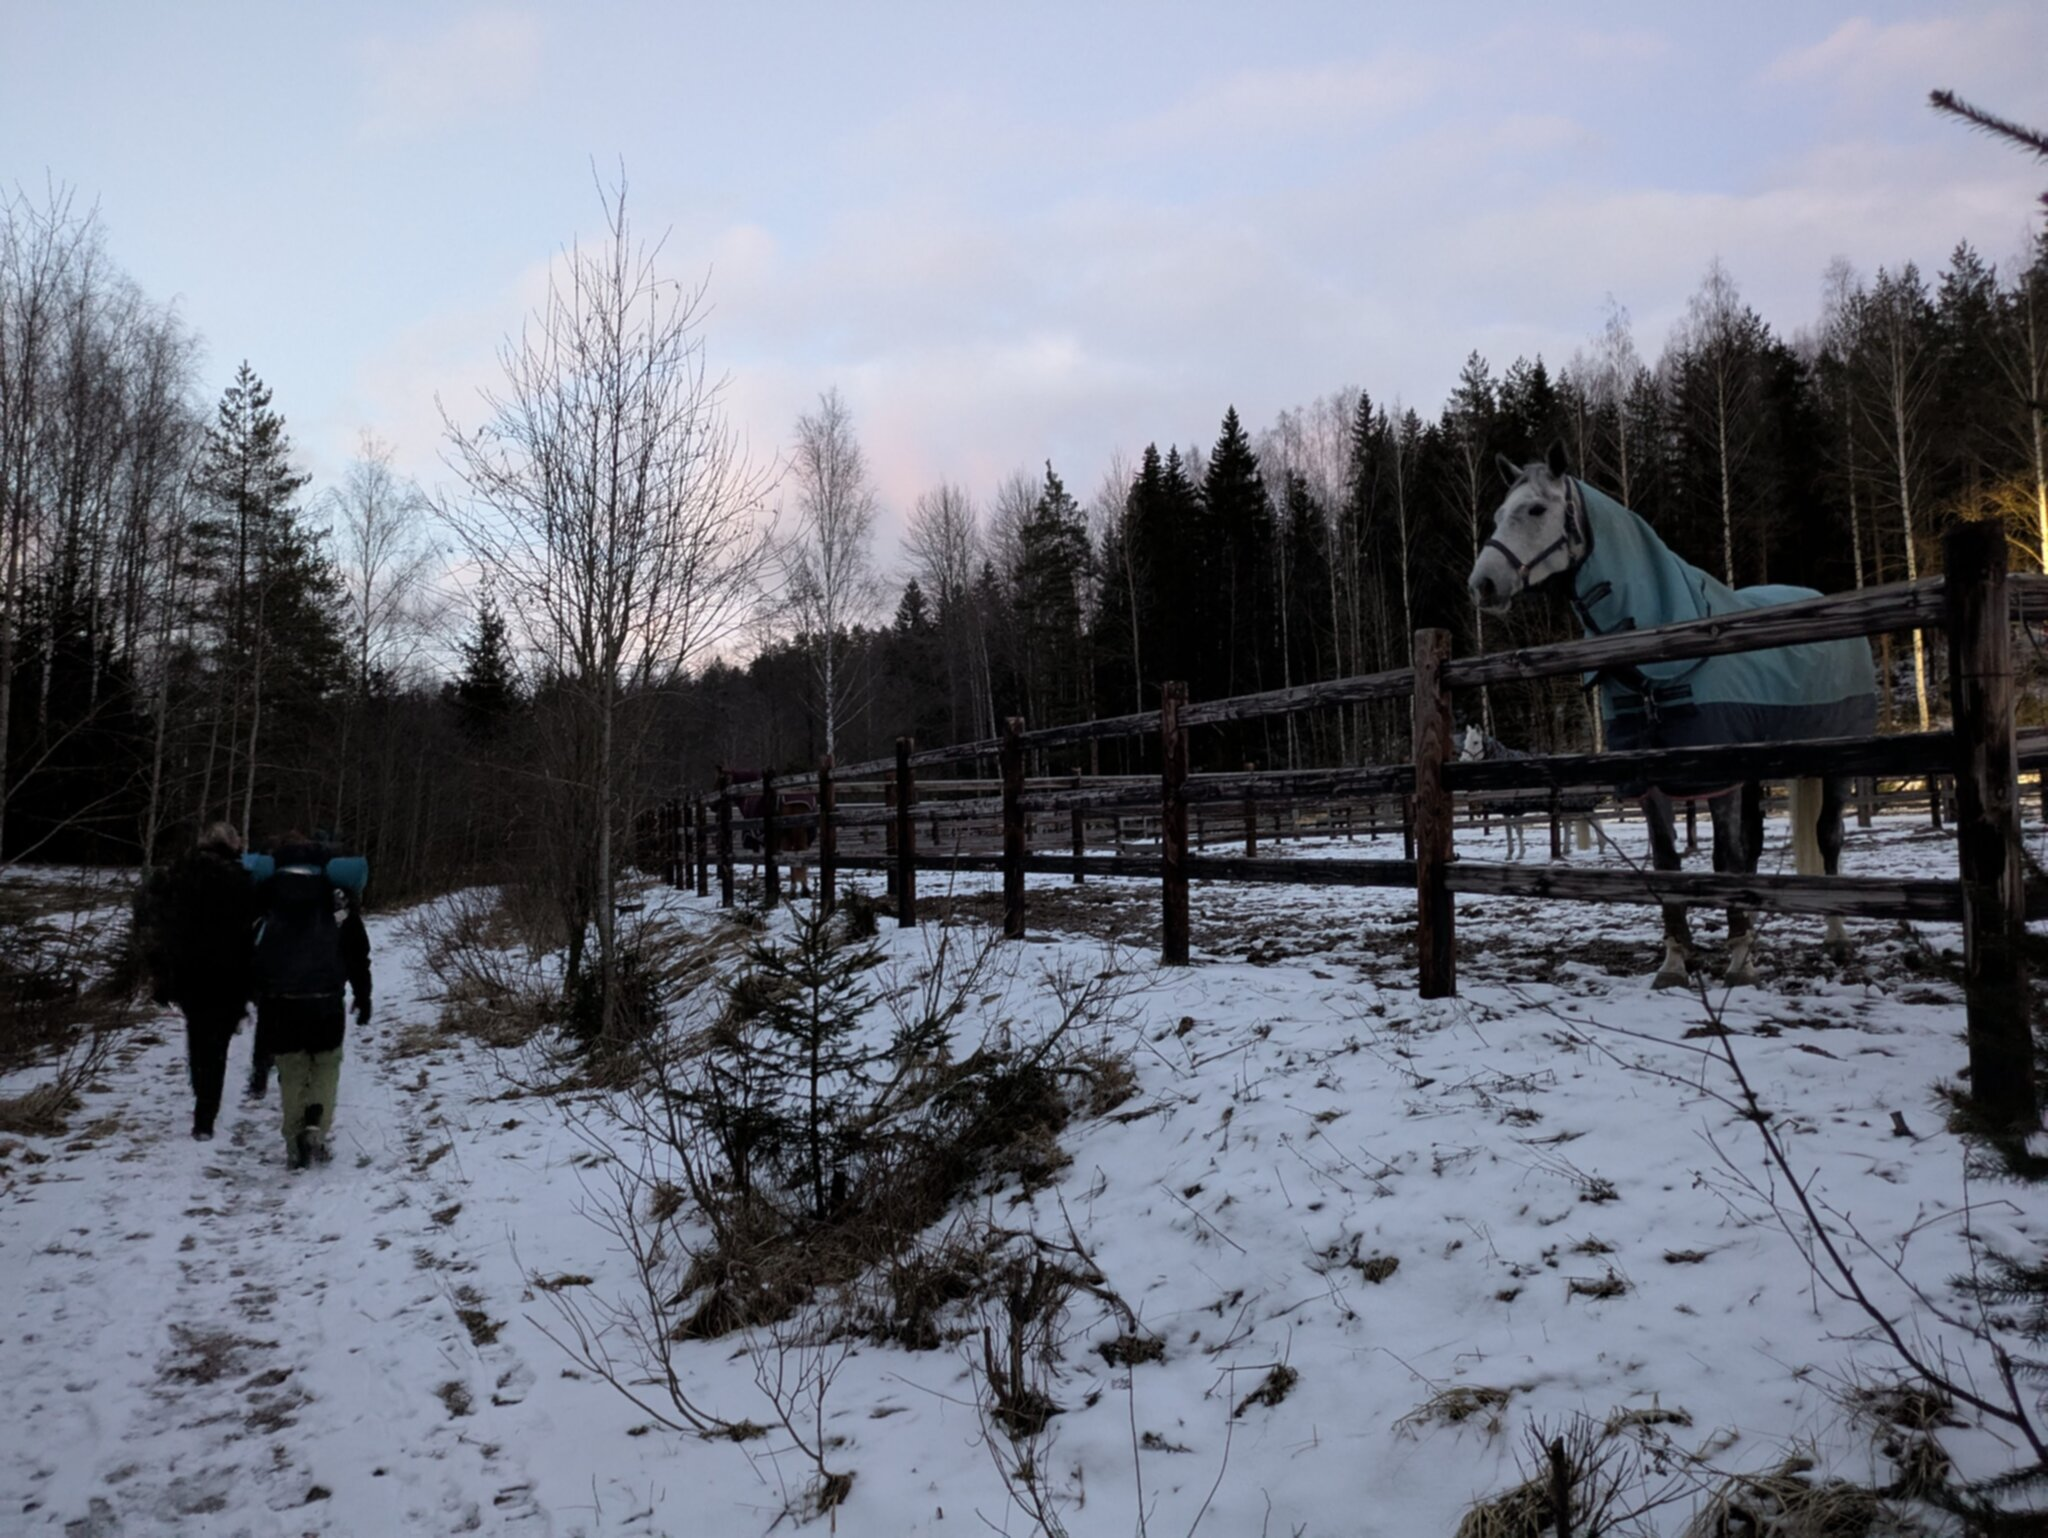
\includegraphics[width=1.0\linewidth,trim={0 10cm 0 10cm},clip]{assets/minihaikki1}

\vspace*{-0.32cm}
\noindent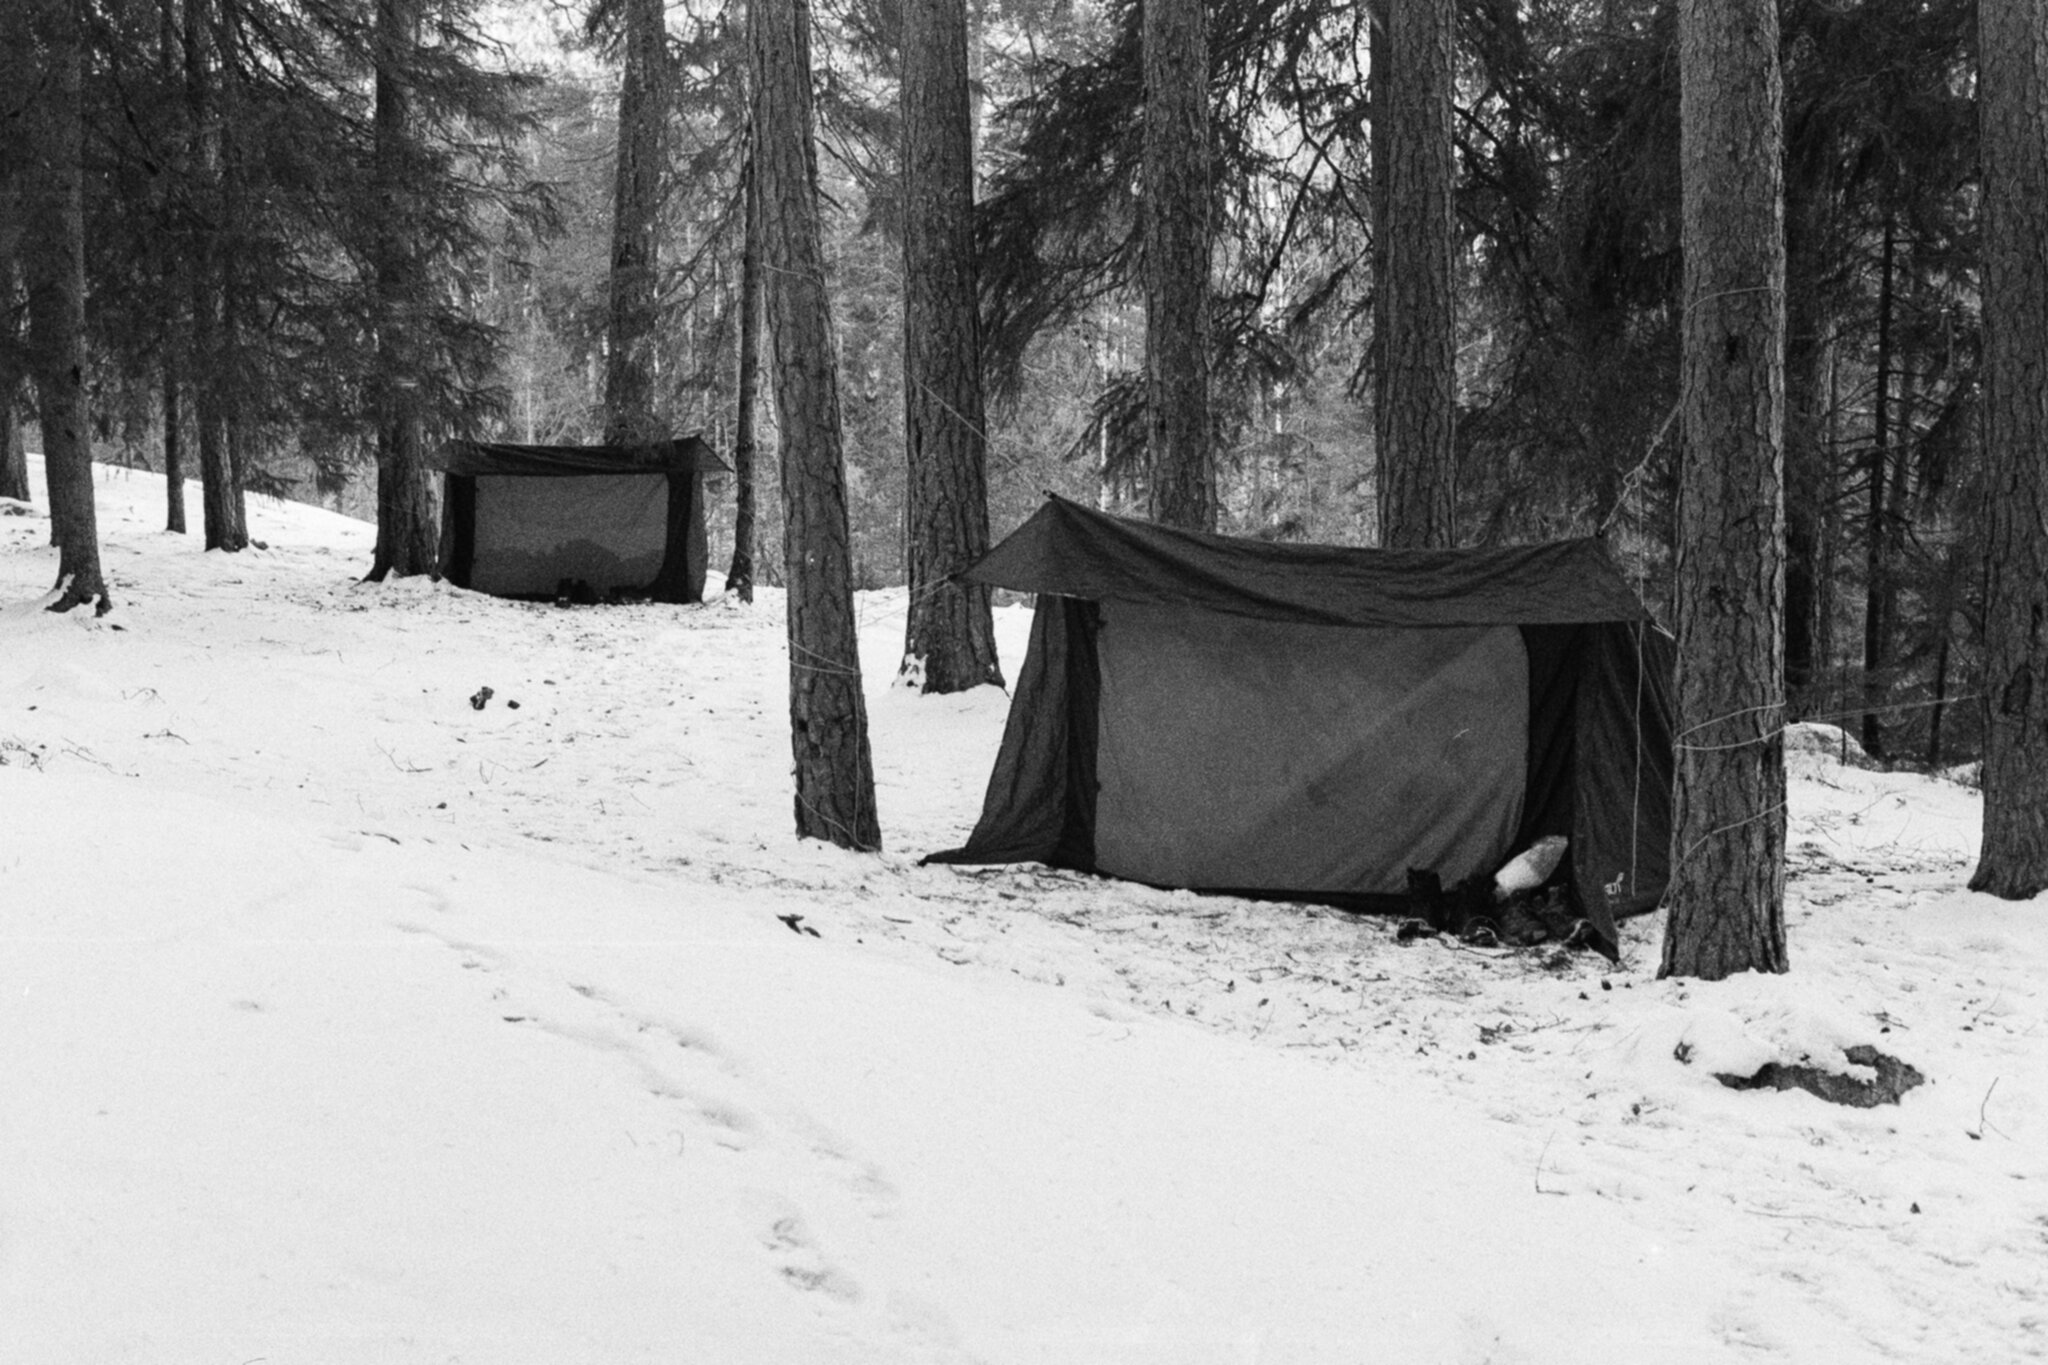
\includegraphics[width=1.0\linewidth,trim={0 2cm 0 2cm},clip]{assets/minihaikki2}

\noindent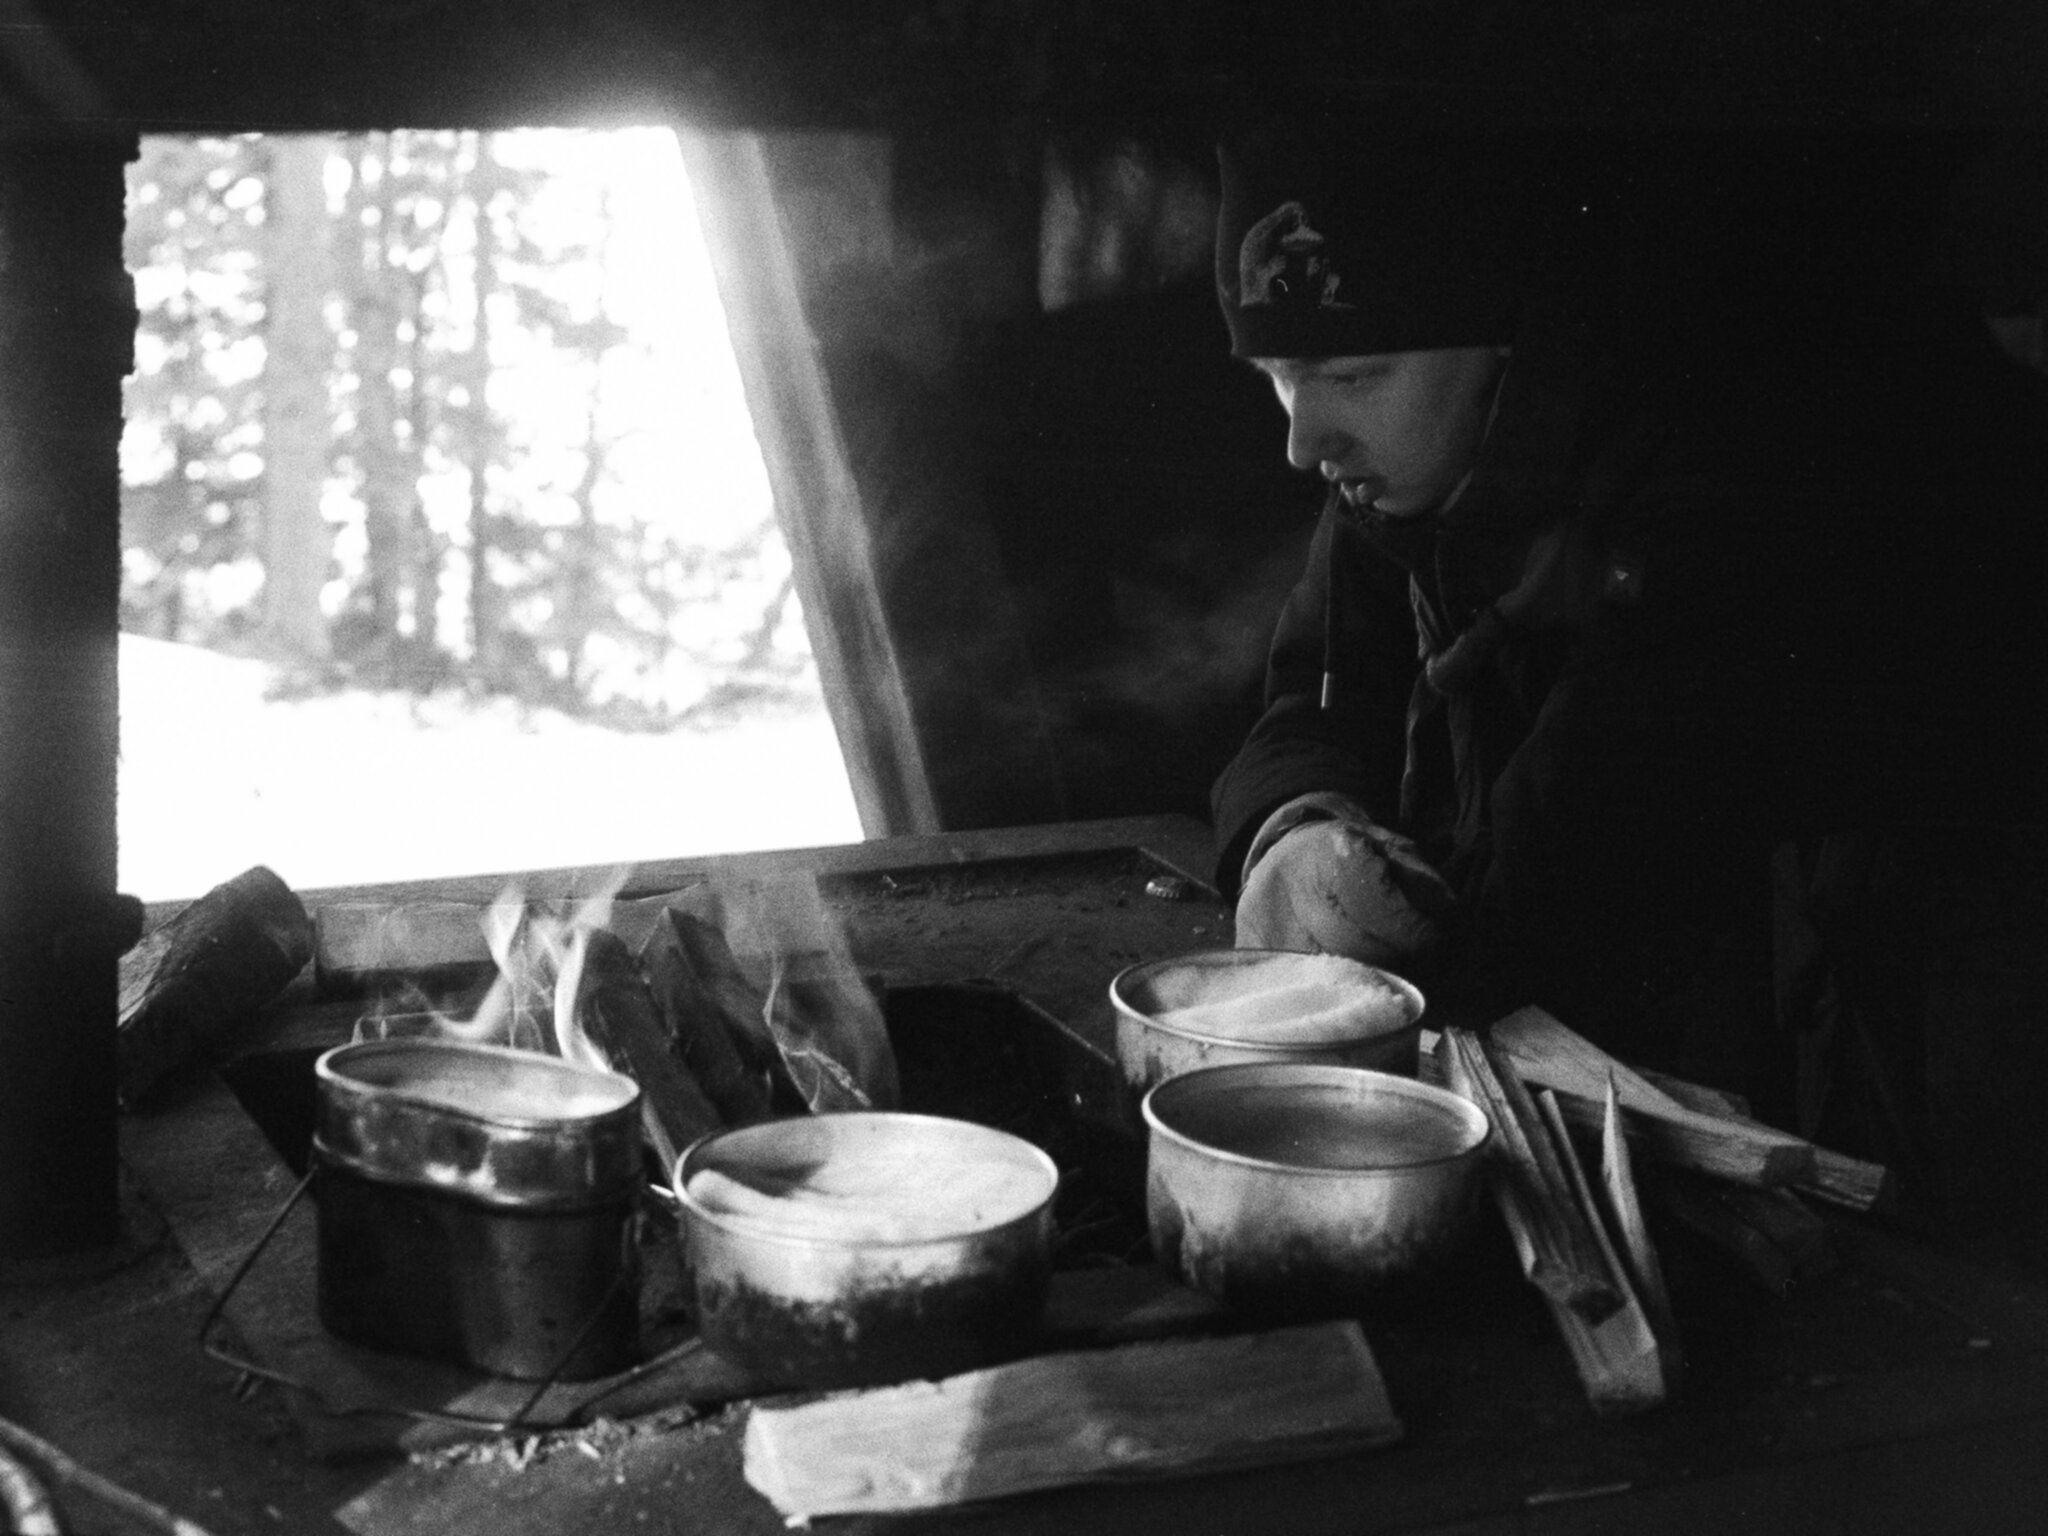
\includegraphics[width=1.0\linewidth,trim={0 0 0 0},clip]{assets/minihaikki3}

Aamulla herätessä todettiin, että sääennuste oli hyvinkin pitänyt paikkansa,
sillä ainakin allekirjoittanut voi todeta, että kylmyys tosiaan kiusasi. Yöllä
oltiin vältytty lumisateelta, mutta aamulla lämpötilan noustessa kosteus oli
hiipinyt sisään telttaan, jolloin varusteet olivat kostuneet. Aamupalalla
sitten kuivateltiin varusteita nuotion ääressä, puuroa, kahvia ja Oivallusta
nautiskellen. Pian olikin jo aika purkaa majoitteet ja jatkaa matkaa.
Ensimmäisen suunnistusvuoron sai Leo, joka pienen harhailun jälkeen sai
suunnistettua porukan lounaspaikalle. Noin kahden kilometrin kävelyn jälkeen
retkikunta pysähtyi Kattilajärventien varrelle valmistamaan lounasta.
Trangioilla valmistui herkullinen “ranskalainen” sipulikeitto, jonka mausteena
toimi kuivattu sipuli. Ja mitä olisikaan ateria ilman Oivallusta ja kahvia!
Lautaset tyhjinä ja energiaa täyteen tankattuina retkeilijät lähtivät tarpomaan
kohti seuraavaa etappia, Urja-järveä. Seuraavan suunnistusvuoron sai Alden,
joka sunnistikin onnistuneesti muutaman kilometrin matkan Urjalle, jonka
rannalla sijaitsikin jo seuraava yöpaikka. Matkalla päiviteltiin jälleen
seuraavan yön sääennustetta, joka vaikutti aiempaakin yötä karmeammalta. Yksi
aste lämmintä ja räntää…

\bigskip
\noindent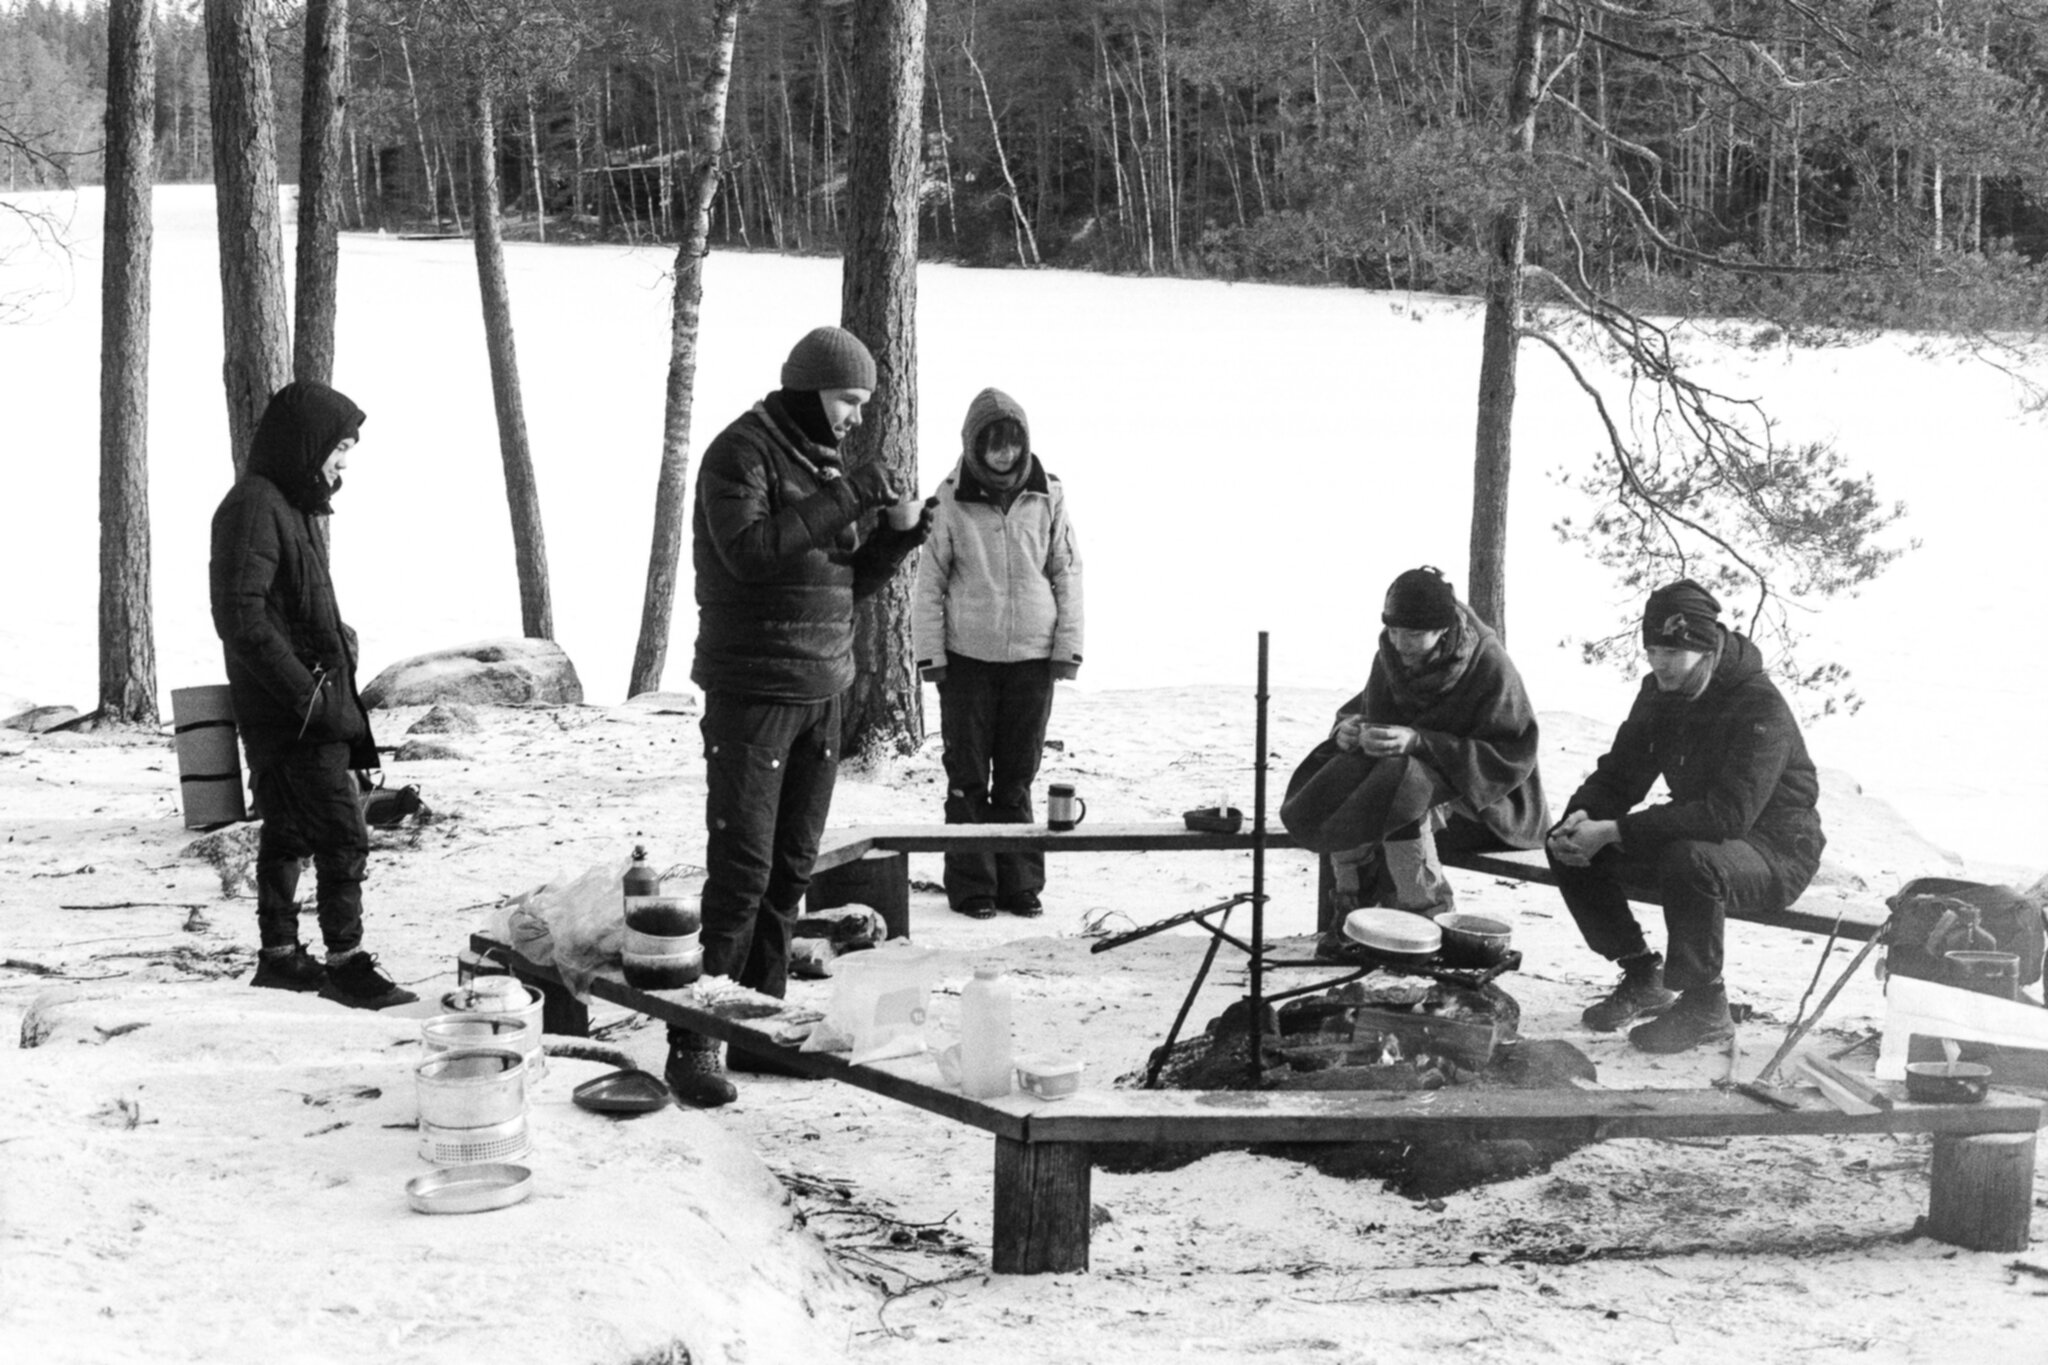
\includegraphics[width=1.0\linewidth,trim={0 0 0 0},clip]{assets/minihaikki6}
\smallskip

Urjalle saavuttaessa todettiin, ettei laavupaikan löytäminen ollut yhtään niin
helppoa kuin Hynkänlammella ja sopivia paikkoja etsittiin miltei puoli tuntia.
Kun paikat löytyivät ja majoitteet saatiin kasaan, oli jälleen ruoka-aika.
Koska Urjalla oli rusakoiden lisäksi muitakin retkeilijöitä, jotka olivat
miehittäneet nuotiopaikan, täytyi retkikunnan valmistaa ruokaa trangialla.
Iltaruuaksi syötiin tomaattista soijapataa sekä salami-tomaattipastaa.
Kasvisruokailijoiden harmiksi soijanpalaset maistuivat pitkälti pahvilta, mutta
siitä huolimatta vatsat saatiin täyteen. Loppuilta kuluikin yhdessä aikaa
viettäessä ja jutellessa. Iltapalana oli Hönöä, Oivallusta, Lämmintä kuppia ja
teetä. Illan pimentyessä ja kylmetessä retkikunta painui nukkumaan.

\vfill*
\columnbreak

\begin{center}
\noindent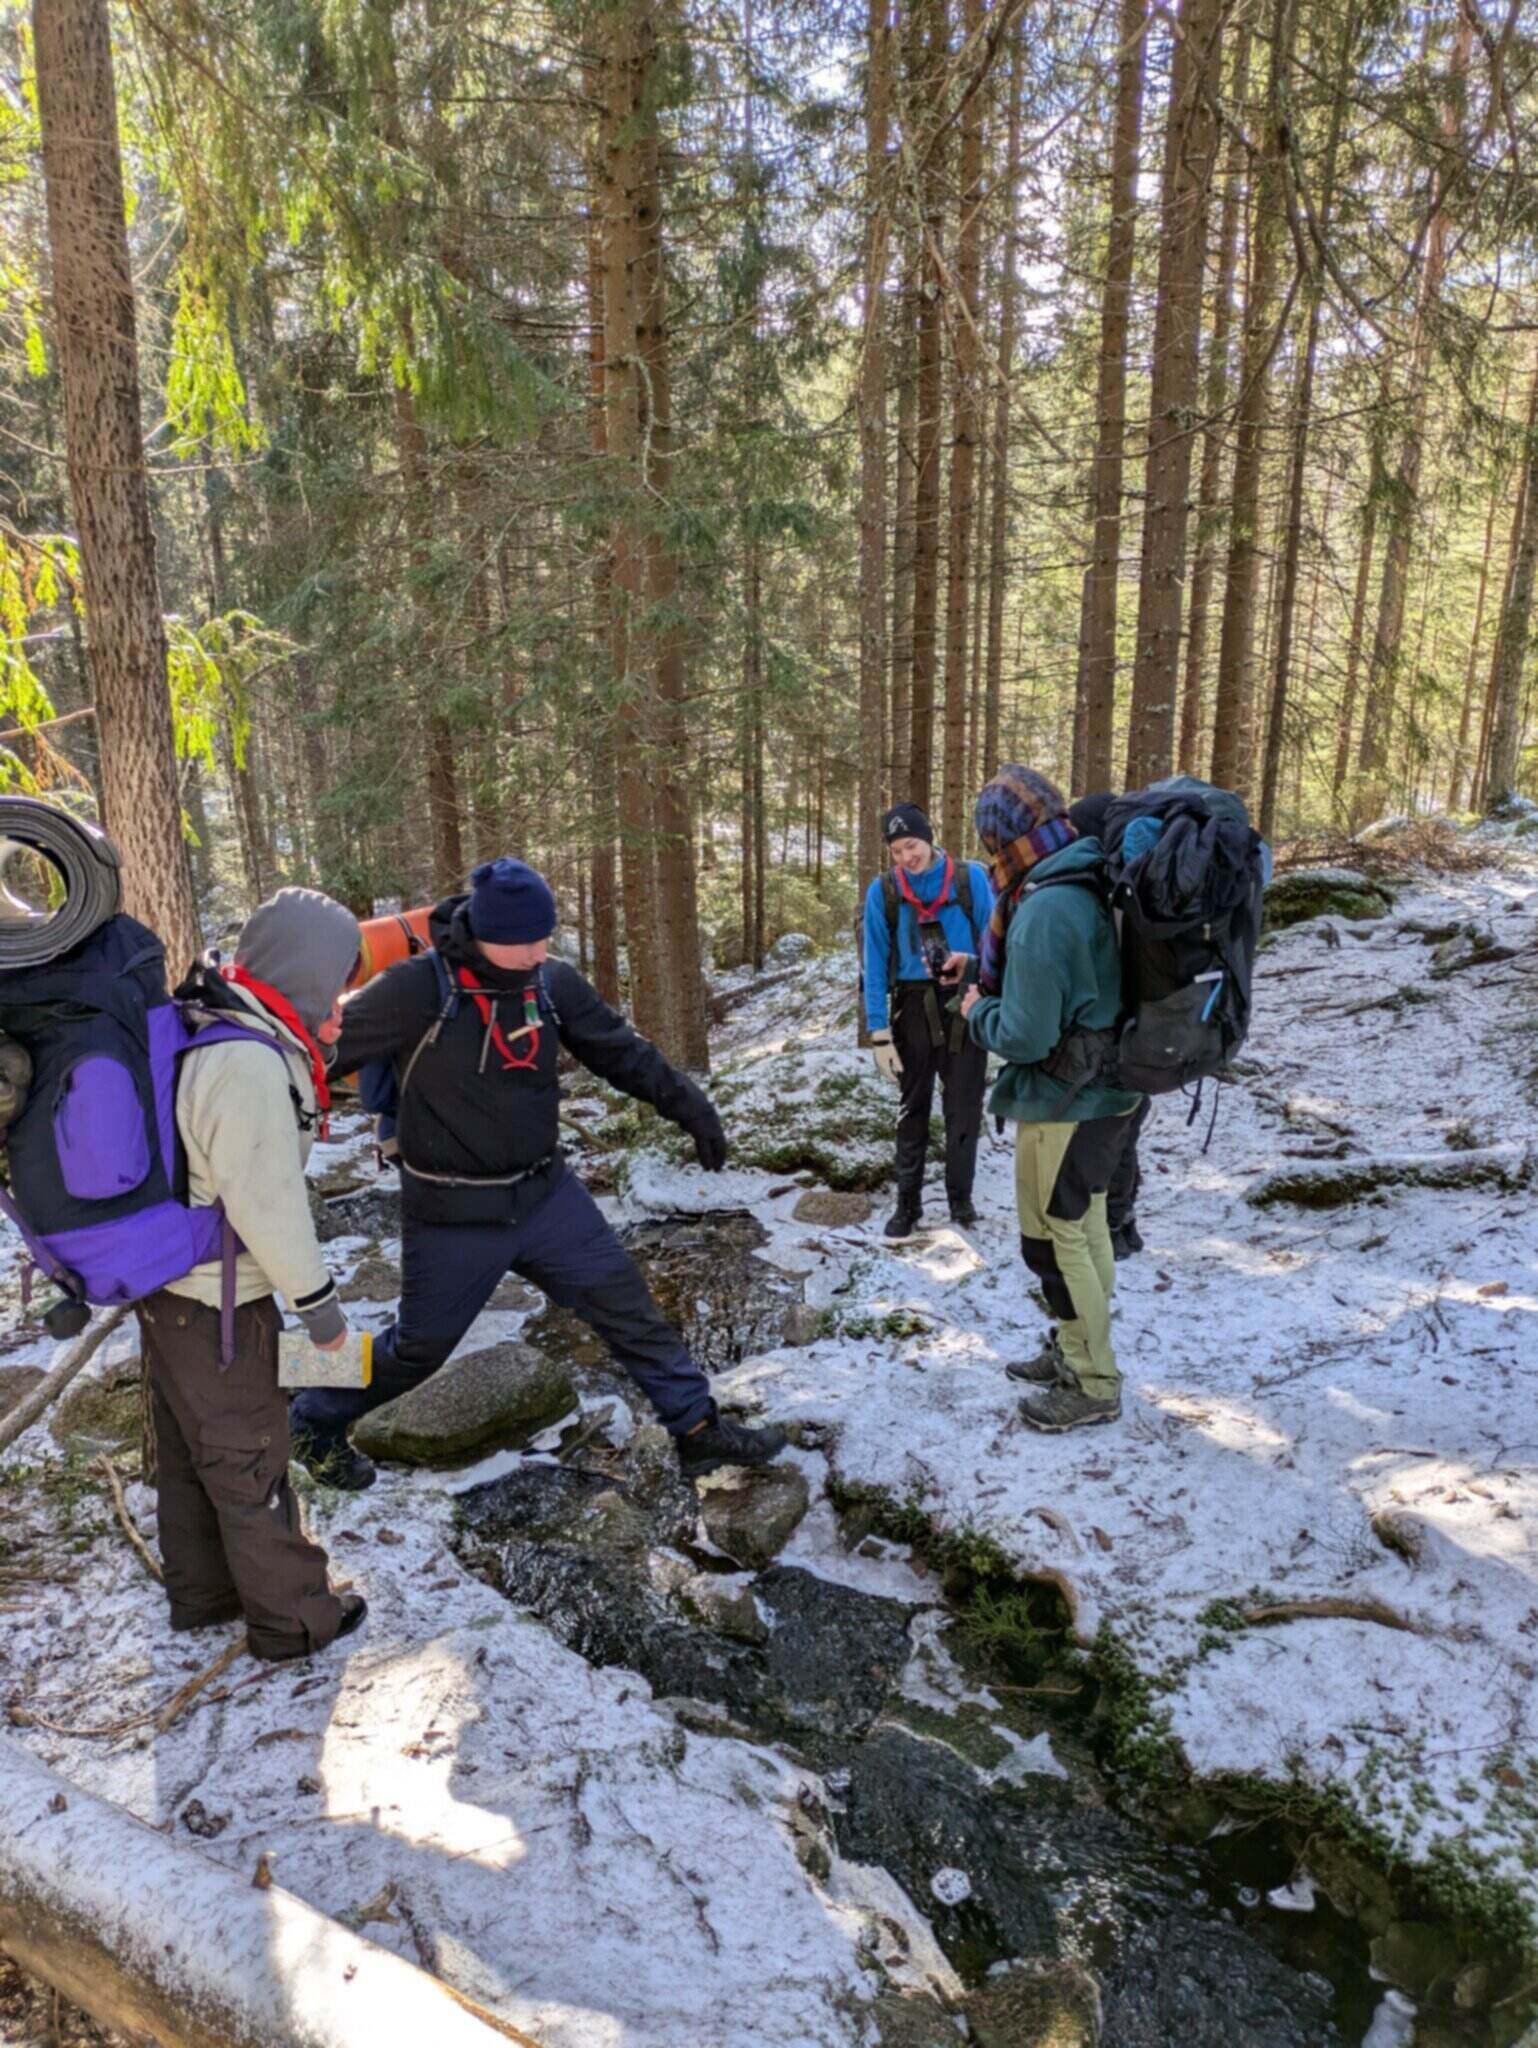
\includegraphics[width=1.0\linewidth,trim={0 0 0 0},clip]{assets/minihaikki5}
\end{center}

Haikin viimeinen aamu alkoi kosteissa tunnelmissa. Sääennuste oli totta tosiaan
pitänyt paikkansa ja yön räntäsade oli tullut läpi laavun katosta. Etenkin
teltan keskiosaan kerätyt tavarat kuten allekirjoittaneen toppatakki olivat
kastuneet. Onneksi muulta seurueelta sai kuivaa vaatetta lainaan, minkä lisäksi
aamupuuro ja -kahvi sekä nuotio lämmittivät aamun kylmyydessä. Aamiaisen
jälkeen oli vielä aika tiskata astiat, pakata loput tavarat ja purkaa
majoitteet, minkä jälkeen matka pääsi jatkumaan. Suunnistusvuoron sai nyt
puolestaan Tesla, jonka tehtävänä oli suunnistaa seurue Haltiaan
bussipysäkille. Matkalla päädyttiin kuitenkin tekemään pieni poikkeus, kun
retkikunta päätti lähteä katsomaan Meerlammen luolaa. Matkalla luolalle
ylitettiin pieniä vesialueita, listattiin suomen kielen mö-alkuisia sanoja ja
nautittiin auringonpaisteesta, jota oli kaivattu koko viikonlopun ajan.

Meerlammella todettiin, että “luola” on hiukan harhaanjohtava termi paikalla
olevista kallioista ja suurista siirtolohkareista. Se oli kuitenkin mukava
levähdyspaikka ja sen kivimuodostelman alla saatiin otettua myös retken
virallinen yhteiskuva. Meerlammen nähtävyyksien jälkeen matka jatkui kohti
Haltiaa. Matkalla aloitettiin jälleen uusi kielellinen haaste, kun retkikunta
alkoi keksimään tulevan kesän vaellukselle v-kirjaimella alkavia nimiä.
Juomaveden loppuessa osa alkoi maistella Nuuksion purojen virtavesien
tarjontaa, mikä herätti muissa hiukan ihmetystä. Lopulta saavuttiin Haltiaan,
jolloin todettiin koko minihaikin matkasaldoksi yksitoista kilometriä.
245A-bussia saatiin odotella jonkin aikaa, jolloin oli hyvin aikaa käydä vielä
vessassa Haltian luontokeskuksessa. Bussimatka saatiin jakaa kahden muun
Nuuksiossa retkeilleen lippukunnan kanssa tupaten täydessä bussissa. Espoon
keskuksesta lähdettiin E-junalla kohti kotia. Ikävistä sääolosuhteista
huolimatta retki oli onnistunut ja seurue jälleen valmiina uusiin
seikkailuihin.
\columnbreak

\noindent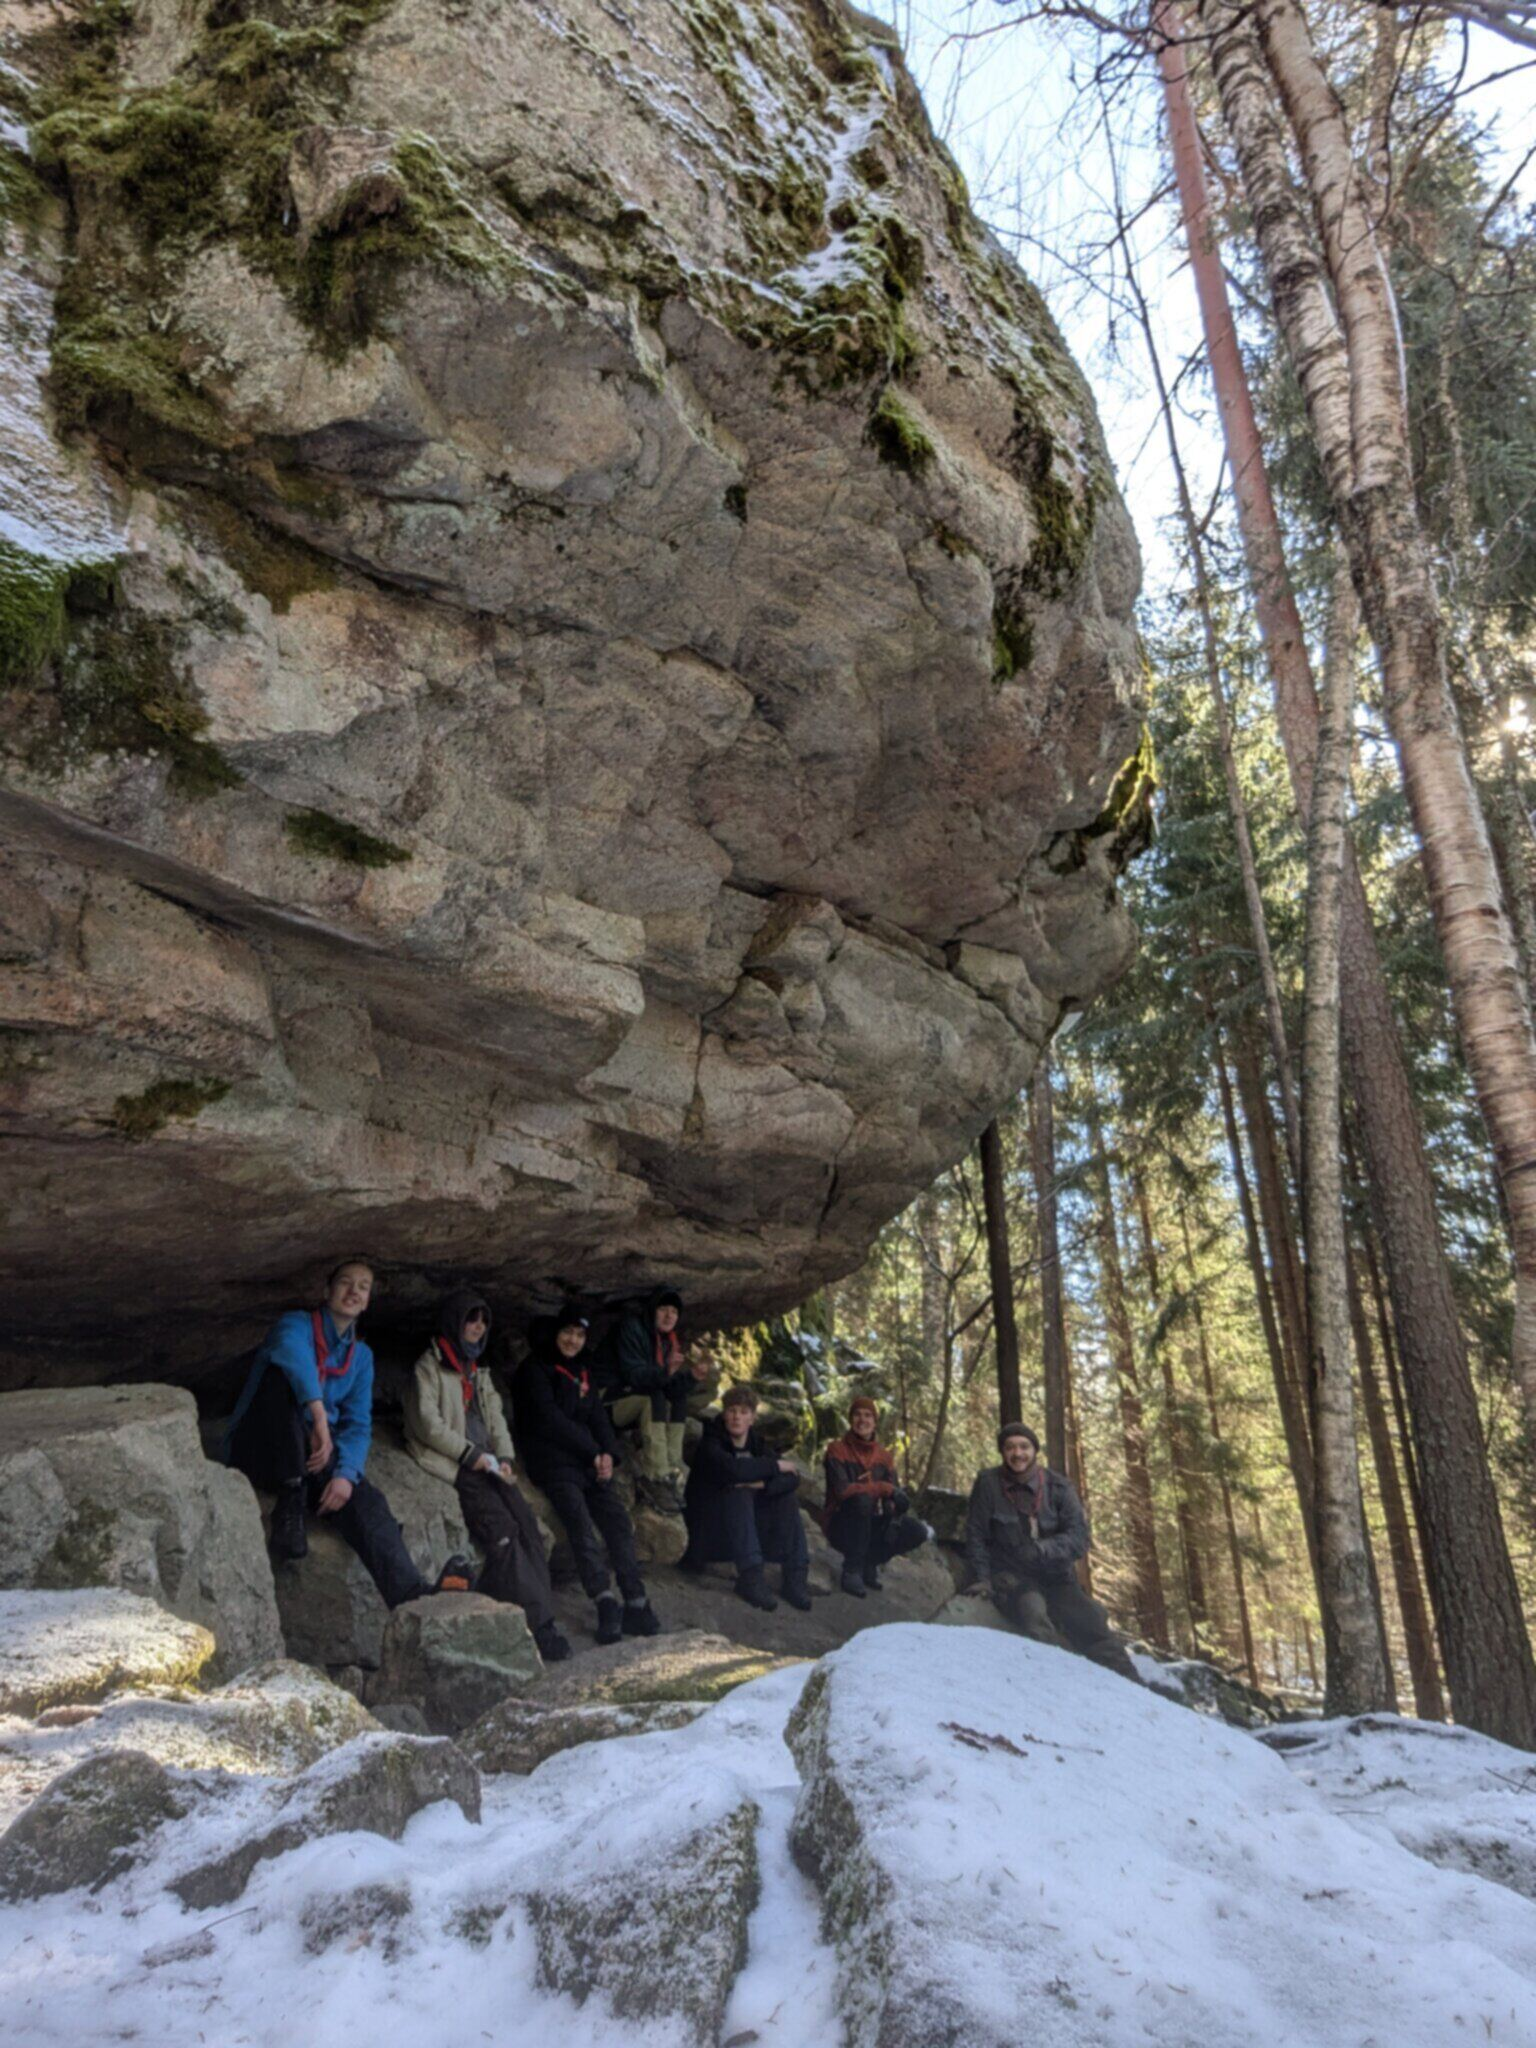
\includegraphics[width=1.2\linewidth,trim={4cm 0 6cm 0},clip]{assets/minihaikki7}

\end{multicols}


\noindent\null\hfill Kuvat: Tanguy\\
\noindent\null\hfill Teksti: Leo
